%%
% Please see https://bitbucket.org/rivanvx/beamer/wiki/Home for obtaining beamer.
%%
\documentclass[aspectratio=169, table,colorlinks]{beamer}
\usetheme{Madrid}

%% COLOR
\usepackage{fontawesome}
\definecolor{newred}{rgb}{0.8,0,0}
\definecolor{avocado}{HTML}{2B7A0B}
\definecolor{newblue}{HTML}{0270c0}


%\definecolor{avocado}{RGB}{88,172,91}

%% THEME
\setbeamertemplate{navigation symbols}{}
\setbeamertemplate{headline}{}
\setbeamercolor{footer}{fg=white, bg=avocado}
\usecolortheme[named=avocado]{structure}
\makeatletter
\setbeamertemplate{footline}
{
  \leavevmode%
  \hbox{%
  \begin{beamercolorbox}[wd=\paperwidth,ht=2.25ex,dp=1ex,left]{footer}%
    \hspace*{2ex}\usebeamerfont{author in head/foot}\insertshortauthor\hspace{0pt plus 1 filll} \insertframenumber{} \hspace*{2ex} 
  \end{beamercolorbox}}%
  \vskip0pt%
}
\makeatother
\setbeamertemplate{blocks}[rounded][shadow=false]
\addtobeamertemplate{footline}{\hypersetup{allcolors=.}}{}
\addtobeamertemplate{title page}{\hypersetup{allcolors=.}}{}

\setbeamertemplate{title page}{%
\hypersetup{allcolors=.}
    \begin{tikzpicture}[remember picture,overlay]
    \node[anchor = east, xscale=-1, yscale = 1] at (current page.west) {\includegraphics[width=\paperwidth]{img/background.jpg}};
    \node[inner xsep=20pt, inner ysep=20pt, minimum width = 0.7\paperwidth, text width=0.7\paperwidth, align = left, text = avocado, anchor = north west] at (current page.north west) (aff){\includegraphics[height = 1.3cm]{img/iiflogo.png}\hspace{0.5cm}\includegraphics[height = 1.3cm]{img/F4SGLogo.png}\hspace{0.5cm}\includegraphics[height = 1.3cm]{img/unipd800.png}};
    \draw[line width=0.5 mm, color = newblue] ([yshift=-0.45cm]current page.west) -- ([yshift=-0.45cm, xshift=-5.5cm]current page.east);
    \node[inner xsep=20pt, inner ysep=10pt, minimum width = 0.7\paperwidth, text width=0.7\paperwidth, align = left, anchor=west, text=avocado, execute at begin node=\setlength{\baselineskip}{6ex}] at ([yshift=0.75cm]current page.west) (title2){\usebeamerfont{title}\huge\textbf{\inserttitle}};
    \node[inner xsep=20pt, inner ysep=20pt, minimum width = 0.7\paperwidth, text width=0.7\paperwidth, align = left, text = black, anchor = south west] at (current page.south west) (auth){{\usebeamerfont{author}\large\textbf{Daniele Girolimetto}}\\[2mm]
    {\footnotesize\begin{tabular}{cl}
    	\faCloud & \href{https://danigiro.github.io/}{danigiro.github.io}\\
    	\faGithub & \href{https://github.com/daniGiro}{github.com/daniGiro}\\
    	\faAt & \href{mailto:daniele.girolimetto@phd.unipd.it}{daniele.girolimetto@phd.unipd.it}\\
    \end{tabular}}\\[2mm]
    {\small\usebeamerfont{author}Department of Statistical Sciences, University of Padova (Italy)}\\[2mm]
    {\small\usebeamerfont{author}\textbf{March 31$^{st}$, 2023}}};
    \end{tikzpicture}
}

\hypersetup{allcolors=newblue}

%% TABLE
\usepackage{booktabs}
\newcolumntype{M}[1]{>{\centering\arraybackslash}m{#1}}
\newcolumntype{L}[1]{>{\raggedright\arraybackslash}m{#1}}
\newcolumntype{R}[1]{>{\raggedleft\arraybackslash}m{#1}}


%% ITEMIZE
\setbeamercolor{itemize item}{fg=black}
\setbeamertemplate{itemize item}[square]
\setbeamertemplate{itemize subitem}[circle]
\setbeamertemplate{itemize subsubitem}[triangle]


\setbeamercolor{enumerate item}{fg=black}
\setbeamertemplate{enumerate item}[circle]
\setbeamertemplate{sections/subsections in toc}[square]
\setbeamertemplate{section in toc}[sections numbered]

\usepackage{enumitem}
\setitemize{label=\usebeamerfont*{itemize item}%
	\usebeamercolor[fg]{itemize item}
	\usebeamertemplate{itemize item}}
\setlist[enumerate,1]{%
	label=\protect\usebeamerfont{enumerate item}%
	\protect\usebeamercolor[fg]{enumerate item}%
	\insertenumlabel.%
}

%% TIKZ
\usepackage{tikz}
\usetikzlibrary{arrows, shapes, positioning, shadows, backgrounds, trees, shapes.misc, arrows.meta, calc, fit}
\tikzset{
  basic/.style  = {draw, text width=2cm, drop shadow, font=\sffamily, rectangle},
  root/.style   = {basic, rounded corners=2pt, thin, align=center,
                   fill=green!30},
  level 2/.style = {basic, rounded corners=6pt, thin,align=center, fill=green!60,
                   text width=4em},
  level 3/.style = {basic, thin, align=left, fill=pink!60, text width=1.5em}
}
\newcommand{\relation}[3]
{
	\draw (#3.south) -- +(0,-#1) -| ($ (#2.north) $)
}
\newcommand{\relationP}[3]
{
	\draw (#3.south) -- +(0,-#1) -| (#2.north)
}
\newcommand{\relationW}[2]
{
	\draw (#2.west) -| ($ (#1.north) $)
}
\newcommand{\relationE}[2]
{
	\draw (#2.east) -| ($ (#1.north) $)
}
\newcommand{\relationD}[3]
{
	\draw (#3.east) -- +(#1,0) |- (#2.west)
}

%% Math symbol
\usepackage{bm}
\newcommand{\avet}{\bm{a}}
\newcommand{\bvet}{\bm{b}}
\newcommand{\cvet}{\bm{c}}
\newcommand{\dvet}{\bm{d}}
\newcommand{\evet}{\bm{e}}
\newcommand{\pvet}{\bm{p}}
\newcommand{\fvet}{\bm{f}}
\newcommand{\tvet}{\bm{t}}
\newcommand{\uvet}{\bm{u}}
\newcommand{\vvet}{\bm{v}}
\newcommand{\wvet}{\bm{w}}
\newcommand{\xvet}{\bm{x}}
\newcommand{\yvet}{\bm{y}}
\newcommand{\zvet}{\bm{z}}
\newcommand{\Avet}{\bm{A}}
\newcommand{\Bvet}{\bm{B}}
\newcommand{\Cvet}{\bm{C}}
\newcommand{\Dvet}{\bm{D}}
\newcommand{\Evet}{\bm{E}}
\newcommand{\Fvet}{\bm{F}}
\newcommand{\Gvet}{\bm{G}}
\newcommand{\Hvet}{\bm{H}}
\newcommand{\Ivet}{\bm{I}}
\newcommand{\Jvet}{\bm{J}}
\newcommand{\Kvet}{\bm{K}}
\newcommand{\Lvet}{\bm{L}}
\newcommand{\Mvet}{\bm{M}}
\newcommand{\Nvet}{\bm{N}}
\newcommand{\Pvet}{\bm{P}}
\newcommand{\Qvet}{\bm{Q}}
\newcommand{\Rvet}{\bm{R}}
\newcommand{\Svet}{\bm{S}}
\newcommand{\Tvet}{\bm{T}}
\newcommand{\Uvet}{\bm{U}}
\newcommand{\Wvet}{\bm{W}}
\newcommand{\Xvet}{\bm{X}}
\newcommand{\Yvet}{\bm{Y}}
\newcommand{\Zvet}{\bm{Z}}
\newcommand{\Zerovet}{\bm{0}}
\newcommand{\Omegavet}{\bm{\Omega}}
\newcommand{\betavet}{\bm{\beta}}
\newcommand{\epsvet}{\bm{\varepsilon}}
\newcommand{\etavet}{\bm{\eta}}

\newcommand\norm[1]{\lVert#1\rVert}


%% NOTES
\usepackage{pgfpages}
%\setbeameroption{show notes on second screen}
\setbeamerfont{note page}{size=\large}
\setbeamertemplate{note page}{\pagecolor{white}
\hspace{-1.5em}\makebox[1.1\textwidth][c]{\begin{minipage}{1.05\linewidth}
		\vbox{}\vskip.25em
{\large \textcolor{black}{\textbf{\insertframetitle}}}\\[-1em]
       \insertnote
	\end{minipage}}
	}

\title{Forecast Reconciliation for \\ Hierarchically Organized Data}
\author{Daniele Girolimetto}

\begin{document}
\begin{frame}[plain, label = titlep]
   \maketitle
\end{frame}

\begin{frame}{Why forecast reconciliation?}
\centering
	\includegraphics[width = \linewidth]{img/gsplot.pdf}\\
	Hot topic in the recent years debate on forecasting methodology and practice: several contributions starting from {\color{newblue}Hyndman et al. (2011)}
\end{frame}


\begin{frame}{What is forecast reconciliation}
\begin{itemize}[itemsep = 0.5cm]
	\item Post-forecasting process aimed to improve the quality of the base forecasts (however obtained) of a {\color{newblue}linearly constrained} multiple time series by exploiting cross-sectional (e.g., spatial) and/or temporal constraints of the {\color{newblue}target} forecasts
	\begin{itemize}
		\item {\color{newblue}cross-sectional} constraints
		\item {\color{newblue}temporal} constraints
		\item {\color{newblue}cross-temporal} constraints (both cross-sectional and temporal)
	\end{itemize}
	 \item Looking for approaches
	\begin{itemize}
		\item {\color{newblue}statistically well-grounded} (interpretation, properties)
		\item {\color{newblue}feasible}, for practical implementation
		\item {\color{newblue}effective}, in terms of quality of the results in real-world applications
	\end{itemize}
	\item Forecasting examples: Sales, Production, Tourism, Energy demand, Healthcare, Real estate, Supply chain $\dots$
\end{itemize}	
\end{frame}

\begin{frame}{Linearly constrained multiple time series}{Hierarchical/grouped time series}
\begin{itemize}
	\item A hierarchical time series is a collection of several time series that are linked together in a hierarchical structure (e.g., geographical energy consumption).
	\item A grouped time series is a collection of time series that are aggregated according to multiple hierarchical structures (e.g., tourism flows grouped by region and purpose of travel)
	\item Many forecasting applications involve {\color{newblue}linearly constrained} multiple (not only {\color{newblue}hierarchical/grouped}) time series
\end{itemize}
\vskip0.25cm
\begin{block}{}
	A cross-sectional (contemporaneous) hierarchical/grouped time series is a collection of $n$ variables for which - at each time - \textbf{aggregation relationships} hold. It is
	a special case of \textbf{multiple time series} with exact \textbf{linear constraints}
\end{block}	
\end{frame}

\begin{frame}{Hierarchical, grouped and linearly constrained time series}
\centering
\begin{minipage}{0.49\linewidth}
\centering
\textit{\footnotesize Hierarchical time series}\\[0.1cm]
\resizebox{0.6\linewidth}{!}{
		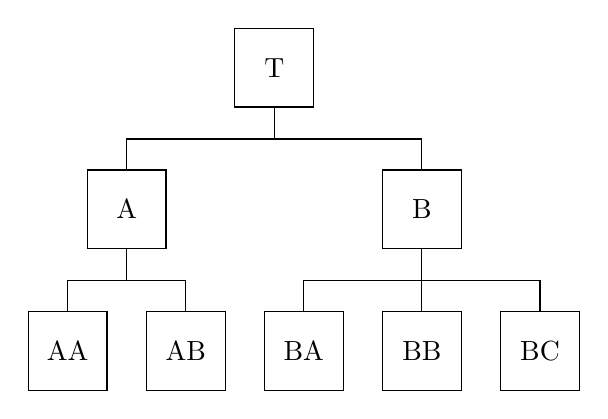
\begin{tikzpicture}[baseline=(current  bounding  box.center),
	every node/.append style={shape=rectangle,
		draw=black},
	minimum width=1cm,
	minimum height=1cm]

	\node at (0, 0) (AA){AA};
	\node at (1.5, 0) (AB){AB};
	\node at (3, 0) (BA){BA};
	\node at (4.5, 0) (BB){BB};
	\node at (6, 0) (BC){BC};
	\node at (0.75, 1.8) (A){A};
	\node at (4.5, 1.8) (B){B};
	\node at (2.625, 3.6) (T){T};
	\relation{0.4}{AA}{A};
	\relation{0.4}{AB}{A};
	\relation{0.4}{BC}{B};
	\relation{0.4}{BA}{B};
	\relation{0.4}{BB}{B};
	\relation{0.4}{A}{T};
	\relation{0.4}{B}{T};
	\end{tikzpicture}}
	\footnotesize
	$\begin{aligned}
		\multicolumn{2}{l}{\textbf{Constraints}}\\[0.1cm]
		\text{T} &= \text{A} + \text{B}\\
		\text{A} &= \text{AA} + \text{AB}\\
		\text{B} &= \text{BA} + \text{BB} + \text{BC}
	\end{aligned}
	$
\end{minipage}\hfill\vline
\begin{minipage}{0.49\linewidth}
\centering
\textit{\footnotesize Linearly constrained time series}\\[0.1cm]
\resizebox{0.6\linewidth}{!}{
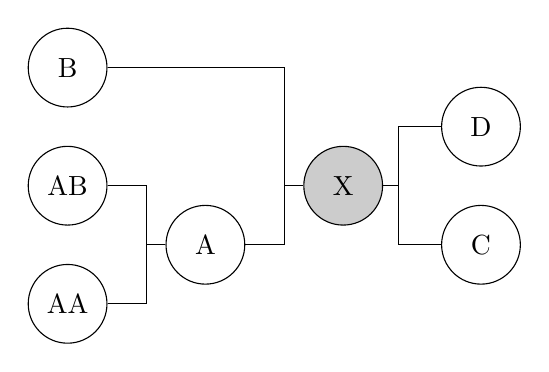
\begin{tikzpicture}[baseline=(current  bounding  box.center),
			rel/.append style={shape=circle,
				draw=black,
			minimum width=1cm,
			minimum height=1cm},
			connection/.style ={inner sep =0, outer sep =0}]
				
			\node[rel] at (0, 0) (A1){AA};
			\node[rel] at (0, 1.5) (A2){AB};
			\node[rel] at (0, 3) (B){B};
			\node[rel] at (5.25, 0.75) (C){C};
			\node[rel] at (5.25, 2.25) (D){D};		
			\node[rel] at (1.75, 0.75) (A){A};
			
			\node[rel, fill = black!20] at (3.5, 1.5) (X){X};
			
			\relationD{0.5}{A}{A1};
			\relationD{0.5}{A}{A2};
			\relationD{0.2}{C}{X};
			\relationD{0.2}{D}{X};
			\relationD{0.5}{X}{A};
			\relationD{2.25}{X}{B};
		\end{tikzpicture}}\hskip0.25cm
	\footnotesize
	$\begin{aligned}
		\multicolumn{2}{l}{\textbf{Constraints}}\\[0.1cm]
		X &= \text{A} + \text{B}\\
		X &= \text{C} + \text{D}\\
		A &= \text{AA} + \text{AB}\\
	\end{aligned}
	$
\end{minipage}
\vskip0.1cm
\hrulefill\\[-1mm]
\textit{\footnotesize Grouped time series}\\
{\footnotesize
\begin{tabular}{c|cc}
	T & \textcolor{newblue}{A} & \textcolor{newblue}{B} \\
	\midrule
	\textcolor{avocado}{Z} & \textcolor{newred}{AZ} & \textcolor{newred}{BZ} \\
	\textcolor{avocado}{Y} & \textcolor{newred}{AY} & \textcolor{newred}{BY}
\end{tabular}}\hspace{0.5cm}
{\large$=$}\hspace{0.25cm}
\resizebox{0.25\linewidth}{!}{
		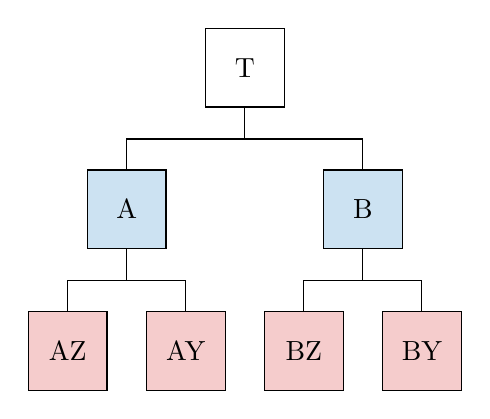
\begin{tikzpicture}[baseline=(current  bounding  box.center),
	every node/.append style={shape=rectangle,
		draw=black},
	minimum width=1cm,
	minimum height=1cm]

	\node[fill = newred, fill opacity = 0.2, text opacity = 1] at (0, 0) (AA){AZ};
	\node[fill = newred, fill opacity = 0.2, text opacity = 1] at (1.5, 0) (AB){AY};
	\node[fill = newred, fill opacity = 0.2, text opacity = 1] at (3, 0) (BA){BZ};
	\node[fill = newred, fill opacity = 0.2, text opacity = 1] at (4.5, 0) (BB){BY};
	\node[fill = newblue, fill opacity = 0.2, text opacity = 1] at (0.75, 1.8) (A){A};
	\node[fill = newblue, fill opacity = 0.2, text opacity = 1] at (3.75, 1.8) (B){B};
	\node at (2.25, 3.6) (T){T};
	\relation{0.4}{AA}{A};
	\relation{0.4}{AB}{A};
	\relation{0.4}{BA}{B};
	\relation{0.4}{BB}{B};
	\relation{0.4}{A}{T};
	\relation{0.4}{B}{T};
	\end{tikzpicture}}
	{\large$+$}
	\resizebox{0.25\linewidth}{!}{
		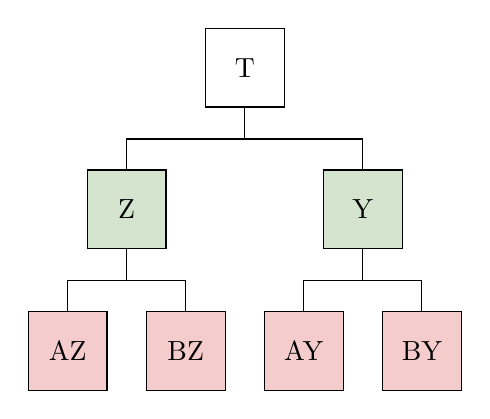
\begin{tikzpicture}[baseline=(current  bounding  box.center),
	every node/.append style={shape=rectangle,
		draw=black},
	minimum width=1cm,
	minimum height=1cm]

	\node[fill = newred, fill opacity = 0.2, text opacity = 1] at (0, 0) (AA){AZ};
	\node[fill = newred, fill opacity = 0.2, text opacity = 1] at (1.5, 0) (AB){BZ};
	\node[fill = newred, fill opacity = 0.2, text opacity = 1] at (3, 0) (BA){AY};
	\node[fill = newred, fill opacity = 0.2, text opacity = 1] at (4.5, 0) (BB){BY};
	\node[fill = avocado, fill opacity = 0.2, text opacity = 1] at (0.75, 1.8) (A){Z};
	\node[fill = avocado, fill opacity = 0.2, text opacity = 1] at (3.75, 1.8) (B){Y};
	\node at (2.25, 3.6) (T){T};
	\relation{0.4}{AA}{A};
	\relation{0.4}{AB}{A};
	\relation{0.4}{BA}{B};
	\relation{0.4}{BB}{B};
	\relation{0.4}{A}{T};
	\relation{0.4}{B}{T};
	\end{tikzpicture}}\hspace{0.5cm}
	{	\footnotesize
	$\begin{aligned}
		\multicolumn{2}{l}{\textbf{Constraints}}\\[0.1cm]
		\text{T} &= \text{A} + \text{B}\\
		\text{A} &= \text{AZ} + \text{AY}\\
		\text{B} &= \text{BZ} + \text{BY}\\[0.1cm]
		\text{T} &= \text{Z} + \text{Y}\\
		\text{Z} &= \text{AZ} + \text{BZ}\\
		\text{Y} &= \text{AY} + \text{BY}\\
	\end{aligned}
	$}
\end{frame}


\begin{frame}[label = {cap:aflook}]{\hyperlink{app:aflook}{\color{white}Forecast reconciliation: a first look}}
\vspace{-0.2cm}
\begin{minipage}{0.49\linewidth}
\centering
\resizebox{0.6\linewidth}{!}{
		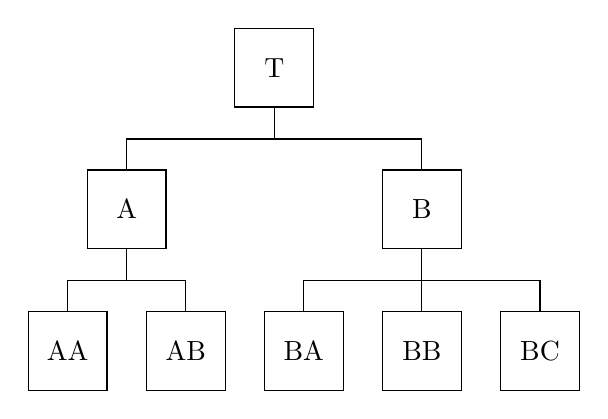
\begin{tikzpicture}[baseline=(current  bounding  box.center),
	every node/.append style={shape=rectangle,
		draw=black},
	minimum width=1cm,
	minimum height=1cm]

	\node at (0, 0) (AA){AA};
	\node at (1.5, 0) (AB){AB};
	\node at (3, 0) (BA){BA};
	\node at (4.5, 0) (BB){BB};
	\node at (6, 0) (BC){BC};
	\node at (0.75, 1.8) (A){A};
	\node at (4.5, 1.8) (B){B};
	\node at (2.625, 3.6) (T){T};
	\relation{0.4}{AA}{A};
	\relation{0.4}{AB}{A};
	\relation{0.4}{BC}{B};
	\relation{0.4}{BA}{B};
	\relation{0.4}{BB}{B};
	\relation{0.4}{A}{T};
	\relation{0.4}{B}{T};
	\end{tikzpicture}}
\end{minipage}
\begin{minipage}{0.49\linewidth}
\centering
\resizebox{0.6\linewidth}{!}{
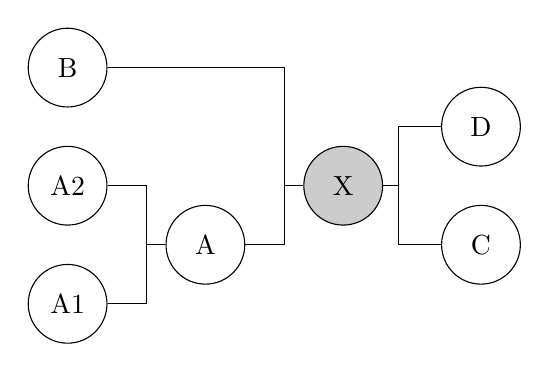
\begin{tikzpicture}[baseline=(current  bounding  box.center),
			rel/.append style={shape=circle,
				draw=black,
			minimum width=1cm,
			minimum height=1cm},
			connection/.style ={inner sep =0, outer sep =0}]
				
			\node[rel] at (0, 0) (A1){A1};
			\node[rel] at (0, 1.5) (A2){A2};
			\node[rel] at (0, 3) (B){B};
			\node[rel] at (5.25, 0.75) (C){C};
			\node[rel] at (5.25, 2.25) (D){D};		
			\node[rel] at (1.75, 0.75) (A){A};
			
			\node[rel, fill = black!20] at (3.5, 1.5) (X){X};
			
			\relationD{0.5}{A}{A1};
			\relationD{0.5}{A}{A2};
			\relationD{0.2}{C}{X};
			\relationD{0.2}{D}{X};
			\relationD{0.5}{X}{A};
			\relationD{2.25}{X}{B};
		\end{tikzpicture}}
\end{minipage}
\hspace{-5cm}
\vskip0.1cm
\begin{minipage}{0.5\linewidth}
	\centering
	$\yvet_t = \begin{bmatrix}
		\Cvet \\ \Ivet_{n_b}
	\end{bmatrix}\bvet_t = \Svet \bvet_t$, {\color{newblue}structural representation}
\end{minipage}\hspace{0.2cm}
\begin{minipage}{0.45\linewidth}
	\centering
		$\Uvet' \yvet_t = 0$, {\color{newblue}zero constrained representation}
\end{minipage}
\vskip0.5cm
\begin{enumerate}
	\item Forecast \textbf{all series at all levels} of aggregation $\rightarrow$ {\color{newred}base forecasts}
	\item Make the base forecasts \textbf{coherent} using least squares $\rightarrow$ {\color{newblue}reconciled forecasts}
\end{enumerate}
\begin{center}
\begin{tabular}{M{0.25\linewidth}M{0.25\linewidth}cM{0.25\linewidth}}
	Target & {\color{newred}Base forecasts} & & Reconciled forecasts \\
	${\Uvet}'\yvet_h = \Zerovet$ & {\color{newred}${\Uvet}'\widehat{\yvet}_h\neq \Zerovet$} & $\rightarrow$ & ${\Uvet}'\widetilde{\yvet}_h = \Zerovet$
\end{tabular}
\vspace{-0.75cm}
\end{center}
\end{frame}

\begin{frame}{Optimal forecast reconciliation}{Wickramasuriya \textit{et al.} (2019), Panagiotelis \textit{et al.} (2021)}
	\begin{block}{}\centering
\vskip0.15cm
	\textbf{Two equivalent point forecast reconciliation formulae}
\vskip0.25cm
\begin{tabular}{M{0.48\linewidth}|M{0.48\linewidth}}
	\textbf{\color{newblue}Structural reconciliation approach} & \textbf{\color{newblue}Projection reconciliation approach} \\
	{\small Structural representation} & {\small Zero-constrained representation} \\[0.25cm]
	$\widehat{\yvet}_h = \Svet \betavet_h + \epsvet_h$ & $\widehat{\yvet}_h = \yvet_h + \epsvet_h,\quad \text{s.t.} \quad \Uvet'\yvet_h = 0$\\[0.2cm]
	$\Downarrow$ & $\Downarrow$ \\[0.2cm]
	$
\widetilde{\yvet}_h = {\Svet}\left({\Svet}'\Wvet^{-1}_h
{\Svet}\right)^{-1}{\Svet}'\Wvet^{-1}_h\widehat{\yvet}_h = \Svet\Gvet\widehat{\yvet}_h
$ & $\widetilde{\yvet}_h =\left[\Ivet - \Wvet_h{\Uvet}\left({\Uvet}’\Wvet_h{\Uvet}\right)^{-1}{\Uvet}'\right]\widehat{\yvet}_h = \Mvet\widehat{\yvet}_h$\\[0.25cm]
\end{tabular}
\end{block}
\vskip0.5cm
	\begin{itemize}
	\item The formulation of $\Wvet_h = \text{E}(\epsvet_h \epsvet_h')$ is conceptually {\color{newred}complex}; in practice, approximate forms are used, possibly using in-sample residuals
\end{itemize}
\end{frame}

\begin{frame}{Temporal hierarchies}{Athanasopoulos et al. (2017), Nystrup et al. (2020)}
\begin{block}{}
A temporal hierarchy is built through \textbf{non-overlapping aggregation} of the observations of a time series at regular intervals
\end{block}
\begin{center}
\resizebox{\linewidth}{!}{
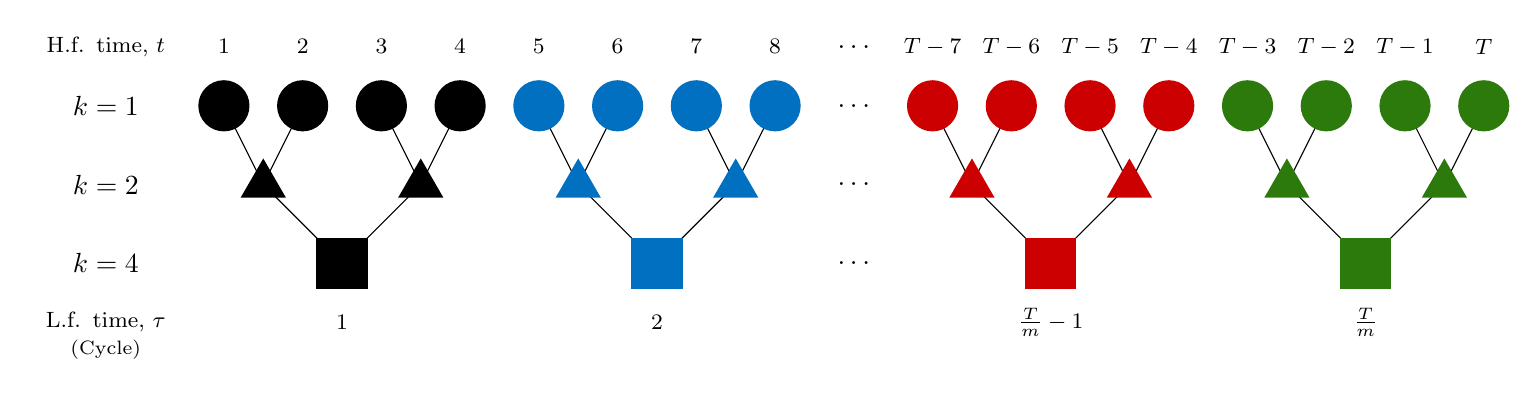
\begin{tikzpicture}
\node[text width = 1.75cm, align = center, anchor = center, font = \footnotesize] at (-1.5,0.75) {H.f. time, $t$};
\node[font = \footnotesize]  at (0,0.75) {1};
\node[font = \footnotesize]  at (1,0.75) {2};
\node[font = \footnotesize]  at (2,0.75) {3};
\node[font = \footnotesize]  at (3,0.75) {4};
\node[font = \footnotesize]  at (4,0.75) {5};
\node[font = \footnotesize]  at (5,0.75) {6};
\node[font = \footnotesize]  at (6,0.75) {7};
\node[font = \footnotesize]  at (7,0.75) {8};
\node at (8,0.75) {$\dots$};
\node[font = \footnotesize] at (9,0.75) {$T-7$};
\node[font = \footnotesize] at (10,0.75) {$T-6$};
\node[font = \footnotesize] at (11,0.75) {$T-5$};
\node[font = \footnotesize] at (12,0.75) {$T-4$};
\node[font = \footnotesize] at (13,0.75) {$T-3$};
\node[font = \footnotesize] at (14,0.75) {$T-2$};
\node[font = \footnotesize] at (15,0.75) {$T-1$};
\node[font = \footnotesize] at (16,0.75) {$T$};
% 1
\foreach \i in {0, 2, 4,6,9, 11,13,15}
	\draw (\i,0) -- (\i+0.5,-1) -- (\i+1,0);
\node at (-1.5,0) {$k = 1$};
\node[circle, fill = black, minimum size = 0.65cm] at (0,0) {};
\node[circle, fill = black, minimum size = 0.65cm] at (1,0) {};
\node[circle, fill = black, minimum size = 0.65cm] at (2,0) {};
\node[circle, fill = black, minimum size = 0.65cm] at (3,0) {};

\node[circle, fill = newblue, minimum size = 0.65cm] at (4,0) {};
\node[circle, fill = newblue, minimum size = 0.65cm] at (5,0) {};
\node[circle, fill = newblue, minimum size = 0.65cm] at (6,0) {};
\node[circle, fill = newblue, minimum size = 0.65cm] at (7,0) {};

\node[circle, minimum size = 0.65cm] at (8,0) {$\dots$};

\node[circle, fill = newred, minimum size = 0.65cm] at (9,0) {};
\node[circle, fill = newred, minimum size = 0.65cm] at (10,0) {};
\node[circle, fill = newred, minimum size = 0.65cm] at (11,0) {};
\node[circle, fill = newred, minimum size = 0.65cm] at (12,0) {};

\node[circle, fill = avocado, minimum size = 0.65cm] at (13,0) {};
\node[circle, fill = avocado, minimum size = 0.65cm] at (14,0) {};
\node[circle, fill = avocado, minimum size = 0.65cm] at (15,0) {};
\node[circle, fill = avocado, minimum size = 0.65cm] at (16,0) {};

% 2
\foreach \i in {0.5, 4.5, 9.5, 13.5}
	\draw (\i,-1) -- (\i+1,-2) -- (\i+2,-1);
\node at (-1.5,-1) {$k = 2$};
\node[regular polygon, regular polygon sides=3, fill = black, minimum size = 0.65cm] at (0.5,-1) {};
\node[regular polygon, regular polygon sides=3, fill = black, minimum size = 0.65cm] at (2.5,-1) {};

\node[regular polygon, regular polygon sides=3, fill = newblue, minimum size = 0.65cm] at (4.5,-1) {};
\node[regular polygon, regular polygon sides=3, fill = newblue, minimum size = 0.65cm] at (6.5,-1) {};

\node[regular polygon, regular polygon sides=3, minimum size = 0.65cm] at (8,-1) {$\dots$};

\node[regular polygon, regular polygon sides=3, fill = newred, minimum size = 0.65cm] at (9.5,-1) {};
\node[regular polygon, regular polygon sides=3, fill = newred, minimum size = 0.65cm] at (11.5,-1) {};

\node[regular polygon, regular polygon sides=3, fill = avocado, minimum size = 0.65cm] at (13.5,-1) {};
\node[regular polygon, regular polygon sides=3, fill = avocado, minimum size = 0.65cm] at (15.5,-1) {};

% 4
\node at (-1.5,-2) {$k = 4$};
\node[rectangle, fill = black, minimum size = 0.65cm] at (1.5,-2) {};
\node[rectangle, fill = newblue, minimum size = 0.65cm] at (5.5,-2) {};
\node[rectangle, minimum size = 0.65cm] at (8,-2) {$\dots$};
\node[rectangle, fill = newred, minimum size = 0.65cm] at (10.5,-2) {};
\node[rectangle, fill = avocado, minimum size = 0.65cm] at (14.5,-2) {};

\node[font = \footnotesize] at (1.5,-2.75) {1};
\node[font = \footnotesize] at (5.5,-2.75) {2};
\node[font = \footnotesize] at (10.5,-2.75) {$\frac{T}{m}-1$};
\node[font = \footnotesize] at (14.5,-2.75) {$\frac{T}{m}$};
\node[text width = 1.75cm, align = center, anchor = center, font = \footnotesize] at (-1.5,-2.75) {L.f. time, $\tau$};
\node[text width = 1.75cm, align = center, anchor = center, font = \scriptsize] at (-1.5,-3.1) {(Cycle)};
\end{tikzpicture}}\\
{\scriptsize Quarterly time series ($k = 1$) aggregated to semi-annual ($k = 2$) and annual ($k = 4$): $k$ denotes the aggregation order (e.g., $k\in\mathcal{K}=\{4,2,1\}$) and $m$ the frequency of the most disaggregated temporal level (e.g., $m = 4$).}
\end{center}
\end{frame}

\begin{frame}{Temporal reconciliation}
\begin{center}
\begin{tikzpicture}[baseline=(current  bounding  box.center),
every node/.append style={shape=rectangle},
minimum size=0.01cm]

\node[color=black] at (1.25, 1) (Q1){$Q_1$};
\node[color=black] at (5.00, 1) (Q2){$Q_2$};
\node[color=black] at (8.75, 1) (Q3){$Q_3$};
\node[color=black] at (12.5, 1) (Q4){$Q_4$};

\node[color=avocado] at (3.125, 2)  (S1){$S_1$};
\node[color=avocado] at (10.625, 2) (S2){$S_2$};

\node[color=newblue] at (6.875, 3) (A){$Y$};
\relation{0.15}{Q1}{S1};
\relation{0.15}{Q2}{S1};
\relation{0.15}{Q3}{S2};
\relation{0.15}{Q4}{S2};
\relation{0.15}{S1}{A};
\relation{0.15}{S2}{A};
\end{tikzpicture}
\vskip0.2cm
{\scriptsize Quarterly hierarchy: quarterly, {\color{avocado}semi-annual} and {\color{newblue}annual} series}
\end{center}
\vskip0.2cm
\begin{itemize}[itemsep=0.15cm]
	\item Unlike cross-sectional hierarchies, where \textbf{$n$ variables at the same time index} are considered, in temporal hierarchies one deals with \textbf{one variable observed at different frequencies}
	\item {\color{newblue}Structural representation} ($\xvet_{\tau} = \Rvet_1\xvet^{[1]}_{\tau}$) and {\color{newblue}zero constrained representation} ($\Zvet_1'\xvet_{\tau} = \Zerovet_{(k^* \times 1)}$) still hold, and may be alternatively used for reconciliation
\end{itemize}
\end{frame}

\begin{frame}{Cross-sectional $+$ Temporal $=$ Cross-temporal}{A cross-temporal hierarchy of three quarterly time series ($X = W + Z$)}
\vspace{-0.2cm}
\noindent\makebox[\textwidth][c]{\begin{minipage}{0.5\linewidth}
\centering
{\footnotesize cross-sectional $\longrightarrow$ temporal}\\
\end{minipage}\begin{minipage}{0.5\linewidth}
\centering
{\footnotesize temporal $\longrightarrow$ cross-sectional}\\
\end{minipage}}
\vskip0.2cm
\noindent\makebox[\textwidth][c]{\hskip0.3cm\begin{minipage}{0.5\linewidth}
\centering
	\resizebox{0.9\linewidth}{!}{
		\begin{tikzpicture}[baseline=(current  bounding  box.center),
	every node/.append style={shape=ellipse,
		draw=black},
	minimum width=1.2cm,
	minimum height=1.2cm]

	
	\node at (0, 0) (5Q1){$w^{[1]}_1$};
	\node at (1.5, 0) (5Q2){$w^{[1]}_2$};
	\node at (3, 0) (5Q3){$w^{[1]}_3$};
	\node at (4.5, 0) (5Q4){$w^{[1]}_4$};
	\node at (0.75, 1.8) (5SA1){$w^{[2]}_1$};
	\node at (3.75, 1.8) (5SA2){$w^{[2]}_2$};
	\node at (2.25, 3.6) (5A){$w^{[4]}_1$};
	\relation{0.2}{5Q1}{5SA1};
	\relation{0.2}{5Q2}{5SA1};
	\relation{0.2}{5Q3}{5SA2};
	\relation{0.2}{5Q4}{5SA2};
	\relation{0.2}{5SA1}{5A};
	\relation{0.2}{5SA2}{5A};
	\node[draw=none, align=center] at (0.25,3.6) {\Large $W$};
	
	\node at (9.5, 0) (6Q1){$z^{[1]}_1$};
	\node at (11, 0) (6Q2){$z^{[1]}_2$};
	\node at (12.5, 0) (6Q3){$z^{[1]}_3$};
	\node at (14, 0) (6Q4){$z^{[1]}_4$};
	\node at (10.25, 1.8) (6SA1){$z^{[2]}_1$};
	\node at (13.25, 1.8) (6SA2){$z^{[2]}_2$};
	\node at (11.75, 3.6) (6A){$z^{[4]}_1$};
	\relation{0.2}{6Q1}{6SA1};
	\relation{0.2}{6Q2}{6SA1};
	\relation{0.2}{6Q3}{6SA2};
	\relation{0.2}{6Q4}{6SA2};
	\relation{0.2}{6SA1}{6A};
	\relation{0.2}{6SA2}{6A};
	\node[draw=none, align=center] at (9.75,3.6) {\Large $Z$};
	
	\node at (4.75, 9) (7Q1){$x^{[1]}_1$};
	\node at (6.25, 9) (7Q2){$x^{[1]}_2$};
	\node at (7.75, 9) (7Q3){$x^{[1]}_3$};
	\node at (9.25, 9) (7Q4){$x^{[1]}_4$};
	\node at (5.5, 10.8) (7SA1){$x^{[2]}_1$};
	\node at (8.5, 10.8) (7SA2){$x^{[2]}_2$};
	\node at (7, 12.6) (7A){$x^{[4]}_1$};
	\relation{0.2}{7Q1}{7SA1};
	\relation{0.2}{7Q2}{7SA1};
	\relation{0.2}{7Q3}{7SA2};
	\relation{0.2}{7Q4}{7SA2};
	\relation{0.2}{7SA1}{7A};
	\relation{0.2}{7SA2}{7A};
	\node[draw=none, align=center] at (5,12.6) {\Large $X$};
	
	\node[draw=black, fit={(5Q1) (5Q2) (5Q3) (5Q4) (5SA1) (5SA2) (5A)},
	minimum width=8cm,
	minimum height=8cm](U1){};
	\node[draw=black, fit={(6Q1) (6Q2) (6Q3) (6Q4) (6SA1) (6SA2) (6A)},
	minimum width=8cm,
	minimum height=8cm](U2){};
	\node[draw=black, fit={(7Q1) (7Q2) (7Q3) (7Q4) (7SA1) (7SA2) (7A)},
	minimum width=8cm,
	minimum height=8cm](T){};
	\relation{0.3}{U1}{T};
	\relation{0.3}{U2}{T};
	\end{tikzpicture}
	}
\end{minipage}\hskip0.3cm\begin{minipage}{0.55\linewidth}
\centering
	\resizebox{\linewidth}{!}{
		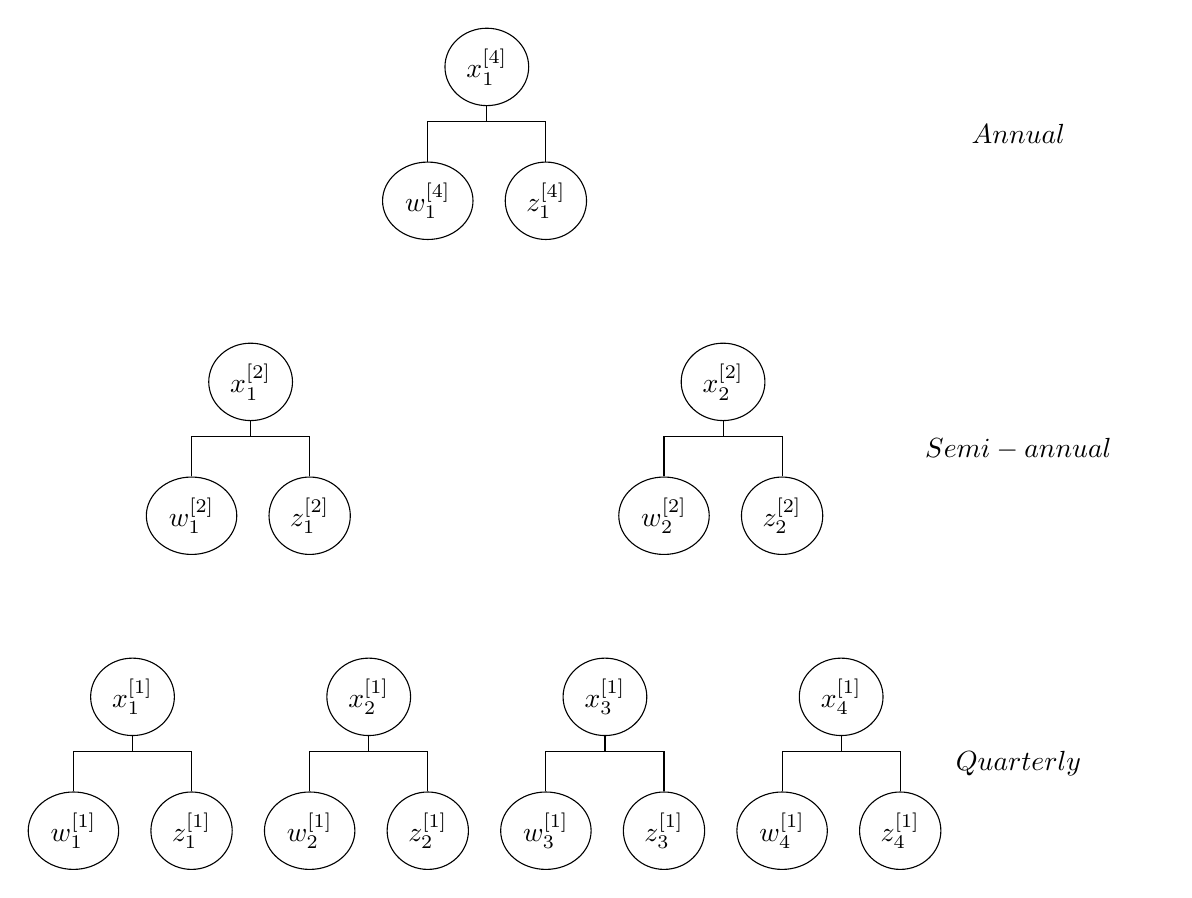
\begin{tikzpicture}[baseline=(current  bounding  box.center),
	every node/.append style={shape=ellipse,
		draw=black}]

	\node at (0, 0) (w1){$w^{[1]}_1$};
	\node at (1.5, 0) (z1){$z^{[1]}_1$};
	\node at (0.75, 1.7) (x1){$x^{[1]}_1$};
	\node at (3, 0) (w2){$w^{[1]}_2$};
	\node at (4.5, 0) (z2){$z^{[1]}_2$};
	\node at (3.75, 1.7) (x2){$x^{[1]}_2$};
	\node at (6, 0) (w3){$w^{[1]}_3$};
	\node at (7.5, 0) (z3){$z^{[1]}_3$};
	\node at (6.75, 1.7) (x3){$x^{[1]}_3$};
	\node at (9, 0) (w4){$w^{[1]}_4$};
	\node at (10.5, 0) (z4){$z^{[1]}_4$};
	\node at (9.75, 1.7) (x4){$x^{[1]}_4$};
	\node[draw=white] at (12, 0.85) (p){$\text{Quarterly}$};
	
	\node at (1.5, 4) (w12){$w^{[2]}_1$};
	\node at (3, 4) (z12){$z^{[2]}_1$};
	\node at (2.25, 5.7) (x12){$x^{[2]}_1$};
	\node at (7.5, 4) (w22){$w^{[2]}_2$};
	\node at (9, 4) (z22){$z^{[2]}_2$};
	\node at (8.25, 5.7) (x22){$x^{[2]}_2$};
	\node[draw=white] at (12, 4.85) (p2){$\text{Semi-annual}$};
	
	\node at (4.5, 8) (w14){$w^{[4]}_1$};
	\node at (6, 8) (z14){$z^{[4]}_1$};
	\node at (5.25, 9.7) (x14){$x^{[4]}_1$};
	\node[draw=white] at (12, 8.85) (p2){$\text{Annual}$};
		
	\relation{0.2}{w1}{x1};
	\relation{0.2}{z1}{x1};
	\relation{0.2}{w2}{x2};
	\relation{0.2}{z2}{x2};
	\relation{0.2}{w3}{x3};
	\relation{0.2}{z3}{x3};
	\relation{0.2}{w4}{x4};
	\relation{0.2}{z4}{x4};
	\relation{0.2}{w12}{x12};
	\relation{0.2}{z12}{x12};
	\relation{0.2}{w22}{x22};
	\relation{0.2}{z22}{x22};
	\relation{0.2}{w14}{x14};
	\relation{0.2}{z14}{x14};
	\end{tikzpicture}
}
\end{minipage}}
\end{frame}

\begin{frame}[label = {cap:ctreco}]{Cross-temporal optimal forecast reconciliation}{Di Fonzo and Girolimetto (2023)}
	\begin{itemize}
	\item The reconciliation formula depends on the \hyperlink{app:ctH}{\color{newblue}full row-rank zero constraints matrix}, $\Hvet'$
	\item $\Hvet'$ is {\color{newred}large} and {\color{newblue}sparse}: function of the {\color{newblue}cross-sectional aggregation matrix} ($\Cvet$) and of the {\color{newblue}frequency of the most disaggregated temporal level} ($m$)
	\item Matrix formulation:
	$$\widehat{\Yvet}_h = \Yvet_h + \Evet \longrightarrow \widehat{\yvet}_h = \yvet_h + \etavet$$
	with $\yvet _h= \text{vec}\left(\Yvet_h'\right)$, $\etavet = \text{vec}\left(\Evet'\right)$ and $\Omegavet = E\left[\etavet\etavet'\right]$
	
	\item {\color{newblue}Projection approach}: 
		$$
		\begin{array}{c}
			\arg \displaystyle\min_{\yvet_h} \left(\widehat{\yvet}_h - \yvet_h\right)' \Omegavet^{-1} \left(\widehat{\yvet}_h - \yvet_h\right) \qquad \text{s.t.} \qquad \Hvet'\yvet_h = \Zerovet\\[0.25cm]
			\Rightarrow\quad \widetilde{\yvet}= \left[\Ivet -\Omegavet\Hvet\left(\Hvet'\Omegavet\Hvet\right)^{-1}\Hvet'\right] \widehat{\yvet} = \Mvet \widehat{\yvet}
		\end{array}
		$$
		\item The {\color{newblue}cross-temporal summing matrix} for the structural representation is $\Svet_{ct} = \Svet \otimes \Rvet_1$
	\end{itemize}
\end{frame}

\begin{frame}{Two-step approach}{Kourentzes and Athanasopoulos, (2019)}
\vspace{-0.2cm}
\begin{center}
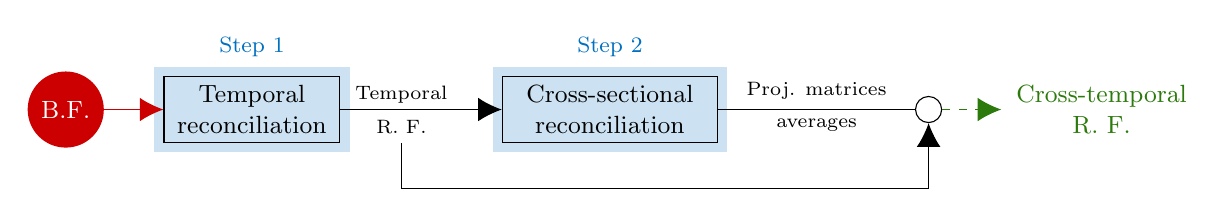
\begin{tikzpicture}
\node[rectangle, draw = black, text width = 2cm, font = \small, align = center] (trec) {Temporal reconciliation};
\node[circle, fill = newred, text = white, font = \small, align = center, left = 0.75cm of trec] (bf) {B.F.};
\node[rectangle, text width = 1.3cm, font = \scriptsize, align = center, right = 0cm of trec] (terec) {Temporal \\[0.15cm] R. F.};
\node[rectangle, draw = black, text width = 2.5cm, font = \small, align = center, right = 0.5cm of terec] (csrec) {Cross-sectional reconciliation};
\node[circle, draw = black, align = center, right = 2.5cm of csrec] (avg) {};
\node[rectangle, text width = 2.3cm, font = \small, align = center, right = 0.75cm of avg, color = avocado] (ctrec) {Cross-temporal \\ R. F.};
\draw (csrec) -- node[above] {\scriptsize Proj. matrices} node[below] {\scriptsize averages} (avg);
\draw[-{Latex[length=3mm, width=3mm]}, color = avocado, dashed] (avg) -- (ctrec);
\draw [-{Latex[length=3mm, width=3mm]}] (terec) -- +(0,-1) -| (avg);
\draw [-{Latex[length=3mm, width=3mm]}, color = newred] (bf) -- (trec);
\begin{pgfonlayer}{background}
\node[fit = (trec), label = above:{\color{newblue}\footnotesize Step 1}, fill = newblue!20] (step1) {} ;
\node[fit = (csrec), label = above:{\color{newblue}\footnotesize Step 2}, fill = newblue!20] (step2) {} ;
\end{pgfonlayer}
\draw[-{Latex[length=3mm, width=3mm]}] (trec) -- (csrec);
\end{tikzpicture}\\
{\scriptsize tcs (KA): first-temporal-then-cross-sectional reconciliation}
\end{center}
\vskip0.1cm
	\begin{itemize}[itemsep=0.15cm, leftmargin = 1.75cm]
	\item[{\color{newred}\bf Step 1}:] reconciliation through temporal hierarchies for each single variable \\ $\qquad\qquad\qquad\rightarrow$ {\color{newblue} temporally coherent} forecasts
	\item[{\color{newred}\bf Step 2}:] time-by-time cross-sectional reconciliation of the previously computed forecasts\\ $\qquad\qquad\qquad\rightarrow$ {\color{newblue} cross-sectionally coherent} forecasts
	\item[{\color{newred}$\bm{\Rightarrow}$}] The final reconciled forecasts are calculated starting from the {\color{newblue}step 1 forecasts} through the average of the {\color{newblue} step 2 projection matrices}\\ $\qquad\qquad\qquad\rightarrow$ {\color{newblue} cross-temporally coherent} forecasts
\end{itemize}
\begin{center} \footnotesize
	\textbf{NB:} Sometimes the average of the projection matrices is not needed (Di Fonzo and Girolimetto, 2022)
\end{center}
\end{frame}

\begin{frame}[label = {cap:ite}]{Iterative cross-temporal point forecast reconciliation}{Alternating point forecast reconciliation along one single dimension (Di Fonzo and Girolimetto, 2022)}
\begin{center}
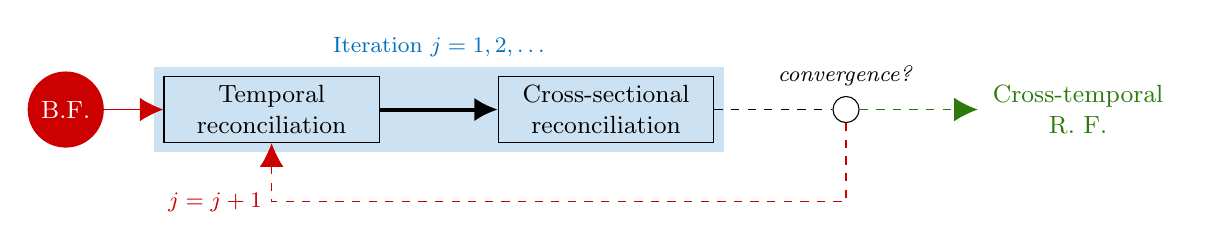
\begin{tikzpicture}
\node[rectangle, draw = black, text width = 2.5cm, font = \small, align = center] (trec) {Temporal reconciliation};
\node[circle, fill = newred, text = white, font = \small, align = center, left = 0.75cm of trec] (bf) {B.F.};
\node[rectangle, draw = black, text width = 2.5cm, font = \small, align = center, right = 1.5cm of trec] (csrec) {Cross-sectional reconciliation};
\node[circle, draw = black, right = 1.5cm of csrec, label = {\footnotesize\textit{convergence?}}] (point) {};
\node[rectangle, text width = 2.3cm, font = \small, align = center, right = 1.5cm of point, color = avocado] (ctrec) {Cross-temporal \\ R. F. };
\draw[-{Latex[length=3mm, width=3mm]}, line width=0.5mm] (trec) -- (csrec);
\draw[dashed] (csrec) -- (point);
\draw[-{Latex[length=3mm, width=3mm]}, color = avocado, dashed] (point) -- (ctrec);
\draw[-{Latex[length=3mm, width=3mm]}, color = newred, dashed] (point.south) -- +(0,-1) -| node[left] {\footnotesize$j = j+1$} (trec.south);
\draw [-{Latex[length=3mm, width=3mm]}, color = newred] (bf) -- (trec);
\begin{pgfonlayer}{background}
\node[fit = (trec)(csrec), label = {\color{newblue}\footnotesize Iteration $j=1,2,\dots$}, fill = newblue!20] {} ;
\end{pgfonlayer}
\end{tikzpicture}\\
{\scriptsize Iterative first-temporal-then-cross-sectional reconciliation}
\end{center}
	\begin{itemize}[itemsep=0.15cm]
	\item {\color{newblue}Each iteration} consists in the {\color{newblue}first two steps} of the heuristic KA procedure, \hyperlink{app:itconv}{\color{newblue}until a convergence criterion} is met. 
	\item {\color{newblue}Quick convergence}, regardless the first fulfilled dimension
	\item Possible {\color{newred}non-negativity constraints} are easily dealt with
	\end{itemize}
\end{frame}

\begin{frame}{Past of reconciliation tools}{in \textbf{\textsf{R}} (R Core Team, 2021)}
\begin{itemize}[topsep = 0mm, itemsep = 2mm, leftmargin = 1.75cm]
	\item[\texttt{hts}] $\rightarrow$ Cross-sectional structural reconciliation (Hyndman et al. 2021). \\
	$\rightarrow$ Available on \href{https://CRAN.R-project.org/package=hts}{\textbf{\textsf{CRAN}}}\\
	$\rightarrow$ \textbf{First release}: 22/03/2010\\
	$\rightarrow$ \textbf{Last release}: 30/05/2021 ({\color{newred}retired on 2020})
	\item[\texttt{thief}] $\rightarrow$ Temporal structural reconciliation (Hyndman and Kourentzes, 2018). \\
	$\rightarrow$ Available on \href{https://CRAN.R-project.org/package=thief}{\textbf{\textsf{CRAN}}}\\
	$\rightarrow$ \textbf{First release}: 07/09/2016\\
	$\rightarrow$ \textbf{Last release}: 24/01/2018
\end{itemize}\vskip0.5cm
\begin{center}
	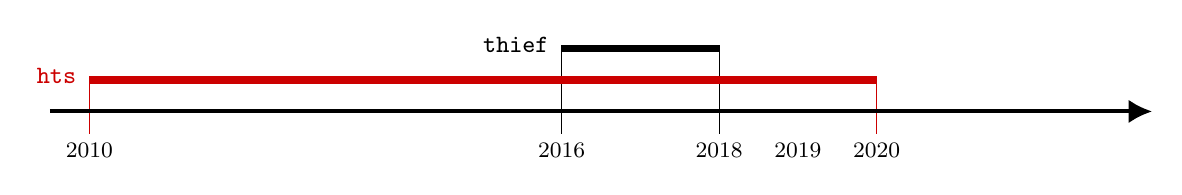
\begin{tikzpicture}
	\node[font = \footnotesize] at (0, -0.5) (t10) {2010};
	\node[font = \footnotesize] at (10, -0.5) (t20) {2020};
	\node[font = \footnotesize] at (9, -0.5) (t19) {2019};
	\node[font = \footnotesize] at (8, -0.5) (t18) {2018};
	\node[font = \footnotesize] at (6, -0.5) (t16) {2016};
	\draw[color = newred] (t10) -- (t10 |- 0,0.45);
	\draw[color = newred] (t20) -- (t20 |- 0,0.45);
	\draw (t18) -- (t18 |- 0,0.85);
	\draw (t16) -- (t16 |- 0,0.85);
	\draw[-{Latex[length=3mm, width=3mm]}, line width=0.5mm] (-0.5,0) -- (13.5,0);
	\draw[line width=1mm, color = newred] (0, 0.4) node[text = black, left, yshift = 0.5mm, font=\small, text = newred] {\texttt{hts}} -- (10, 0.4) ;
	\draw[line width=1mm] (6, 0.8) node[text = black, left, yshift = 0.5mm, font=\small] {\texttt{thief}} -- (8, 0.8);
\end{tikzpicture}
\end{center}
\end{frame}

\begin{frame}{Present and future of reconciliation tools}{in \textbf{\textsf{R}} (R Core Team, 2021)}
\begin{itemize}[topsep = 0mm, itemsep = 2mm, leftmargin = 2.5cm]
	\item[\texttt{fabletools}] $\rightarrow$ new reference for working with time series (O'Hara-Wild et al. 2021). \\
	$\rightarrow$ Only cross-sectional reconciliation is available with \texttt{reconcile()} \\ $\phantom{\rightarrow}$ on \href{https://CRAN.R-project.org/package=fabletools}{\textbf{\textsf{CRAN}}}.\\
	$\rightarrow$ Development version for temporal and cross-temporal reconciliation \\ $\phantom{\rightarrow}$ available on \href{https://github.com/tidyverts/fabletools/tree/temporal}{\textbf{\textsf{GitHub}} \faGithub}. \\
\end{itemize}
\vspace{-0.2cm}
\begin{center}\begin{minipage}{0.8\linewidth}\begin{block}{}
\centering
Waiting for a stable and complete version of \texttt{reconcile()} in \texttt{fabletools}, \texttt{FoReco} is compared with \texttt{hts} and \texttt{thief}.
\end{block} 
\end{minipage}\\[0.2cm]
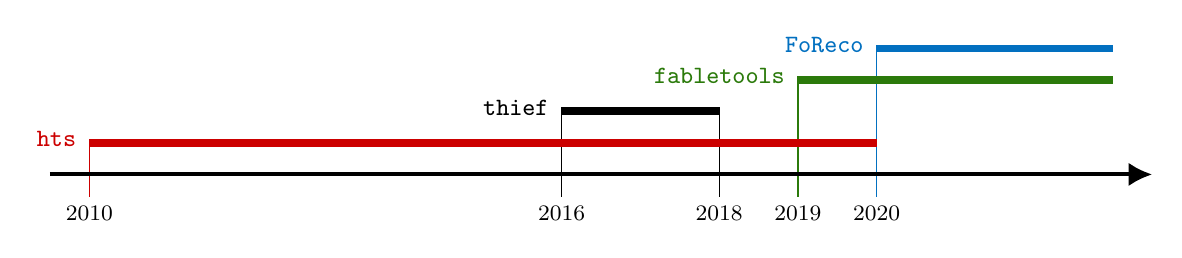
\begin{tikzpicture}
	\node[font = \footnotesize] at (0, -0.5) (t10) {2010};
	\node[font = \footnotesize] at (10, -0.5) (t20) {2020};
	\node[font = \footnotesize] at (9, -0.5) (t19) {2019};
	\node[font = \footnotesize] at (8, -0.5) (t18) {2018};
	\node[font = \footnotesize] at (6, -0.5) (t16) {2016};
	\draw[color = newred] (t10) -- (t10 |- 0,0.45);
	\draw[color = newblue] (t20) -- (t20 |- 0,1.65);
	\draw[color = avocado] (t19) -- (t19 |- 0,1.25);
	\draw (t18) -- (t18 |- 0,0.85);
	\draw (t16) -- (t16 |- 0,0.85);
	\draw[-{Latex[length=3mm, width=3mm]}, line width=0.5mm] (-0.5,0) -- (13.5,0);
	\draw[line width=1mm, color = newred] (0, 0.4) node[text = black, left, yshift = 0.5mm, font=\small, text = newred] {\texttt{hts}} -- (10, 0.4) ;
	\draw[line width=1mm] (6, 0.8) node[text = black, left, yshift = 0.5mm, font=\small] {\texttt{thief}} -- (8, 0.8);
	\draw[line width=1mm, color = avocado] (9, 1.2) node[text = black, left, yshift = 0.5mm, font=\small, text = avocado] {\texttt{fabletools}} -- (13, 1.2);
	\draw[line width=1mm, color = newblue] (10, 1.6) node[text = black, left, yshift = 0.5mm, font=\small, text = newblue] {\texttt{FoReco}} -- (13, 1.6);
\end{tikzpicture}
\end{center}
\end{frame}

\begin{frame}{What is FoReco?}{\textbf{\textsf{R}} package, Di Fonzo and Girolimetto (2022)}
\noindent\makebox[\textwidth][c]{\begin{minipage}{0.6\linewidth}
\centering
   \begin{itemize}[topsep = 0mm, itemsep = 4mm]
	\item FoReco offers classical (bottom-up and top-down), and modern (optimal and heuristic combination) \textbf{\color{newblue}forecast reconciliation procedures} for cross-sectional, temporal, and \textbf{\color{newblue}cross-temporal} \textbf{linearly constrained multiple time series}.
	\item {\color{newred}Matrix-based package}, exploiting the very sparse nature of the involved matrices
	\item \textbf{Links}:
\begin{itemize}
	\item[\mbox{\includegraphics[height = 10pt]{img/rproject.pdf}}] {\small \href{https://cran.r-project.org/package=FoReco}{cran.r-project.org/package=FoReco}}
	\item[\faGithub] {\small \href{https://github.com/daniGiro/FoReco}{github.com/daniGiro/FoReco}}
	\item[\faLeanpub] {\small \href{https://danigiro.github.io/FoReco}{danigiro.github.io/FoReco}}
\end{itemize}
\end{itemize}
\end{minipage}
\begin{minipage}{0.4\linewidth}
\centering
\begin{tabular}{rr}
	\multicolumn{2}{c}{
\includegraphics[width = 0.45\linewidth]{img/logoFoReco.pdf}}\\
	\multicolumn{2}{c}{Available on  \includegraphics[height = 12pt]{img/rproject.pdf}}\\[0.2cm]
	\textbf{First release}: & 01/10/2020\\
	\textbf{Last release}: & 04/07/2022\\
	\textbf{Next release}: & 06/2023\\[0.2cm]
	\multicolumn{2}{c}{\large\textbf{+12k \;\faDownload}}\\
\end{tabular}
\end{minipage}}
\end{frame}

\begin{frame}[plain]
	\begin{tikzpicture}[remember picture,overlay]
    \node[anchor = east, xscale=-1, yscale = 1] at (current page.west) {\includegraphics[width=\paperwidth]{img/background.jpg}};
    \node[inner xsep=20pt, inner ysep=20pt, minimum width = 0.7\paperwidth, text width=0.7\paperwidth, align = left, text = avocado, anchor = north west] at (current page.north west) (aff){\includegraphics[height = 1.3cm]{img/iiflogo.png}\hspace{0.5cm}\includegraphics[height = 1.3cm]{img/F4SGLogo.png}\hspace{0.5cm}\includegraphics[height = 1.3cm]{img/unipd800.png}};
    \draw[line width=0.5 mm, color = newblue] ([yshift=-0.45cm]current page.west) -- ([yshift=-0.45cm, xshift=-5.5cm]current page.east);
    \node[inner xsep=20pt, inner ysep=10pt, minimum width = 0.7\paperwidth, text width=0.7\paperwidth, align = left, anchor=west, text=avocado, execute at begin node=\setlength{\baselineskip}{6ex}] at ([yshift=0.75cm]current page.west) (title2){\usebeamerfont{title}\huge \textbf{What's next? Lab session!}};
    \node[inner xsep=20pt, inner ysep=20pt, minimum width = 0.7\paperwidth, text width=0.7\paperwidth, align = left, text = black, anchor = south west] at (current page.south west) (auth){{\usebeamerfont{author}\large\textbf{Daniele Girolimetto}}\\[2mm]
    {\footnotesize\begin{tabular}{cl}
    	\faCloud & \href{https://danigiro.github.io/}{danigiro.github.io}\\
    	\faGithub & \href{https://github.com/daniGiro}{github.com/daniGiro}\\
    	\faAt & \href{mailto:daniele.girolimetto@phd.unipd.it}{daniele.girolimetto@phd.unipd.it}\\
    \end{tabular}}\\[2mm]
    {\small\usebeamerfont{author}Department of Statistical Sciences, University of Padova (Italy)}\\[2mm]
    {\small\usebeamerfont{author}\textbf{March 31$^{st}$, 2023}}};
    \end{tikzpicture}
\end{frame}

\begin{frame}{References}
\footnotesize
	\begin{itemize}[label = {}, itemindent=-10pt, leftmargin=*]
		\item Athanasopoulos, G., Hyndman, R. J., Kourentzes, N., \& Petropoulos, F. (2017). Forecasting with temporal hierarchies. European Journal of Operational Research, 262, 60–74. \url{https://dx.doi.org/10.1016/j.ejor.2017.02.046}.
		\item Di Fonzo, T. \& Girolimetto, D. (2023), Cross-temporal forecast reconciliation: Optimal combination method and heuristic alternatives, International Journal of Forecasting 39(1), 39– 57. \url{https://doi.org/10.1016/j.ijforecast.2021.08.004}
		\item Di Fonzo, T. \& Girolimetto, D. (2022), Enhancements in cross-temporal forecast reconciliation, with an application to solar irradiance forecasts, \url{https://doi.org/10.48550/arXiv.2209.07146}.
		\item Girolimetto, D. \& Di Fonzo, T. (2022), FoReco: Point Forecast Reconciliation. \url{https://danigiro.github.io/FoReco/}
		\item Hyndman, R. J., Ahmed, R. A., Athanasopoulos, G., \& Shang, H. L. (2011). Optimal combination forecasts for hierarchical time series. Computational Statistics and Data Analysis, 55(9), 2579–2589. \url{https://dx.doi.org/10.1016/j.csda.2011.03.006}.
		\item Hyndman, R. J. e Kourentzes, N. (2018). thief: Temporal HIErarchical Forecasting. url: \url{https://pkg.robjhyndman.com/thief}.
		\item Hyndman, R. J., Lee, A., Wang, E. e Wickramasuriya, S. L. (2021). hts: Hierarchical and Grouped Time Series. url: \url{https://cran.r-project.org/package=hts}.
	\end{itemize}
\end{frame}
\begin{frame}{References}
\footnotesize
	\begin{itemize}[label = {}, itemindent=-10pt, leftmargin=*]
		\item Kourentzes, N., \& Athanasopoulos, G. (2019). Cross-temporal coherent forecasts for Australian tourism. Annals of Tourism Research, 75, 393–409. \url{https://dx.doi.org/10.1016/j.annals.2019.02.001}.
		\item Nystrup, P., Lindstro, E., Pinson, P., \& Madsen, H. (2020). Temporal hierarchies with autocorrelation for load forecasting. European Journal of Operational Research, 280, 876–888. \url{https://dx.doi.org/10. 1016/j.ejor.2019.07.061}.
		\item O'Hara-Wild, M., Hyndman, R.J., and Wang, E. (2021). fabletools: Core Tools for Packages in the 'fable' Framework. url: \url{https://CRAN.R-project.org/package=fabletools}
		\item Panagiotelis, A., Athanasopoulos, G., Gamakumara, P., \& Hyndman, R. J. (2021). Forecast reconciliation: A geometric view with new insights on bias correction. International Journal of Forecasting, 37, 343–359. \url{https://dx.doi.org/10.1016/j.ijforecast.2020.06.004}.
  		\item R Core Team (2021). R: A Language and Environment for Statistical Computing. R Foundation for Statistical Computing. Vienna, Austria. url: \url{https://www.r-project.org/}.
		\item Wickramasuriya, S. L., Athanasopoulos, G., \& Hyndman, R. J. (2019). Optimal forecast reconciliation for hierarchical and grouped time series through trace minimization. Journal of the American Statis- tical Association, 114, 804–819. \url{https://dx.doi.org/10.1080/01621459.2018.1448825}.
	\end{itemize}\vskip0.5cm
	\begin{flushright}\scriptsize
		The cover image has been designed using assets from Freepik.com 
	\end{flushright}
\end{frame}

\appendix
\begin{frame}[label = {app:aflook}]{\hyperlink{cap:aflook}{\color{white}Forecast reconciliation: matrix representations}}
\vspace{-0.2cm}
\begin{minipage}{0.49\linewidth}
\centering
%\begin{minipage}{0.5\linewidth}
\resizebox{0.6\linewidth}{!}{
    $
    \left[\begin{array}{c}
    y_{T,t} \\
	y_{A,t} \\
	y_{B,t} \\
	y_{AA,t} \\
	y_{AB,t} \\
	y_{BA,t} \\
	y_{BB,t} \\
	y_{BC,t}\\
	\end{array}\right]=\left[\begin{array}{ccccc}
1 & 1 & 1 & 1 & 1 \\
1 & 1 & 0 & 0 & 0 \\
0 & 0 & 1 & 1 & 1 \\
1 & 0 & 0 & 0 & 0 \\
0 & 1 & 0 & 0 & 0 \\
0 & 0 & 1 & 0 & 0 \\
0 & 0 & 0 & 1 & 0 \\
0 & 0 & 0 & 0 & 1
\end{array}\right]\left[\begin{array}{c}
	y_{AA,t} \\
	y_{AB,t} \\
	y_{BA,t} \\
	y_{BB,t} \\
	y_{BC,t}\\
	\end{array}\right]
    $}
\end{minipage}
\begin{minipage}{0.49\linewidth}
\centering
%\begin{minipage}{0.5\linewidth}
\resizebox{0.8\linewidth}{!}{
    $
    \left[\begin{array}{ccccccc}
    1 & 0 & 0 & 0 & 0 & -1 & -1 \\
    0 & 1 & 0 & 0 & 1 & -1 & -1 \\
    0 & 0 & 1 & 1 & 1 & -1 & -1
    \end{array}\right]
    \left[\begin{array}{c}
    y_{T,t} \\
	y_{A,t} \\
	y_{A1,t} \\
	y_{A2,t} \\
	y_{B,t} \\
	y_{C,t} \\
	y_{D,t} \\
	\end{array}\right]=\left[\begin{array}{c}
0 \\
	0 \\
	0 \\
	\end{array}\right]
    $}
\end{minipage}
\hspace{-5cm}
\vskip0.1cm
\begin{minipage}{0.5\linewidth}
	\centering
	$\yvet_t = \begin{bmatrix}
		\Cvet \\ \Ivet_{n_b}
	\end{bmatrix}\bvet_t = \Svet \bvet_t$, {\color{newblue}structural representation}
\end{minipage}\hspace{0.2cm}
\begin{minipage}{0.45\linewidth}
	\centering
		$\Uvet' \yvet_t = 0$, {\color{newblue}zero constrained representation}
\end{minipage}
\vskip0.5cm
\begin{enumerate}
	\item Forecast \textbf{all series at all levels} of aggregation $\rightarrow$ {\color{newred}base forecasts}
	\item Make the base forecasts \textbf{coherent} using least squares $\rightarrow$ {\color{newblue}reconciled forecasts}
\end{enumerate}
\begin{center}
\begin{tabular}{M{0.25\linewidth}M{0.25\linewidth}cM{0.25\linewidth}}
	Target & {\color{newred}Base forecasts} & & Reconciled forecasts \\
	${\Uvet}'\yvet_h = \Zerovet$ & {\color{newred}${\Uvet}'\widehat{\yvet}_h\neq \Zerovet$} & $\rightarrow$ & ${\Uvet}'\widetilde{\yvet}_h = \Zerovet$
\end{tabular}
\vspace{-0.75cm}
\end{center}
\end{frame}

\begin{frame}[label = {app:ctH}]{\hyperlink{cap:ctreco}{\color{white}$\Hvet'$: cross-temporal full row-rank zero constraints matrix}}
		$$
	\Yvet_{\tau} = \begin{bmatrix} \xvet_{\tau}' \\ \wvet_{\tau}' \\ \zvet_{\tau}' \end{bmatrix} \quad 
	\Zvet_1' = \begin{bmatrix} 1 & 0 & 0 & -1 & -1 & -1 & -1 \\
			                   0 & 1 & 0 & -1 & -1 &  0 &  0 \\
			                   0 & 0 & 1 &  0 &  0 & -1 & -1 \end{bmatrix} \quad
	\Ivet^* = \begin{bmatrix} 0 & 0 & 0 & 1 & 0 & 0 & 0 \\
			                  0 & 0 & 0 & 0 & 1 & 0 & 0 \\
			                  0 & 0 & 0 & 0 & 0 & 1 & 0 \\
			                  0 & 0 & 0 & 0 & 0 & 0 & 1 \end{bmatrix}
	$$

	$$
		\begin{bmatrix}
		\Ivet^* & -\Ivet^* & -\Ivet^* \\
		\Zvet_1' & \Zerovet & \Zerovet \\
		\Zerovet & \Zvet_1' & \Zerovet \\
		\Zerovet & \Zerovet & \Zvet_1'		
		\end{bmatrix}\text{vec}\left(\Yvet_{\tau}'\right) = \Zerovet \longrightarrow \Hvet'\yvet_\tau = \Zerovet
			$$
\end{frame}

\begin{frame}[label = {app:itconv}]{\hyperlink{cap:ite}{\color{white}Iterative convergence criterion}}{Temporal and the cross-sectional incoherence}
	\begin{itemize}
		\item $L_1$-norm
		$$d_{cs} = \norm{\Uvet'\widehat{\Yvet}}_1 \qquad \text{and} \qquad d_{te} = \norm{\Zvet_1'\widehat{\Yvet}'}_1$$
		with $$\norm{\Xvet}_1 = \sum_{i,j}|x_{i,j}|$$
		\item $L_\infty$-norm
		$$d_{cs} = \norm{\Uvet'\widehat{\Yvet}}_\infty \qquad \text{and} \qquad d_{te} = \norm{\Zvet_1'\widehat{\Yvet}'}_\infty$$
		with $$\norm{\Xvet}_\infty = \max |x_{i,j}|$$
	\end{itemize}

\end{frame}

\begin{frame}{Hourly grouped time series: two temporal hierarchies}{\scriptsize$\mathcal{K} = \{24,12,8,6,3,2,1\}$}
\centering
{\scriptsize Temporal hierarchy $\{24, {\color{newblue}8, 4, 2}, 1\}$}\\[-0.2cm]
\resizebox{\linewidth}{!}{
	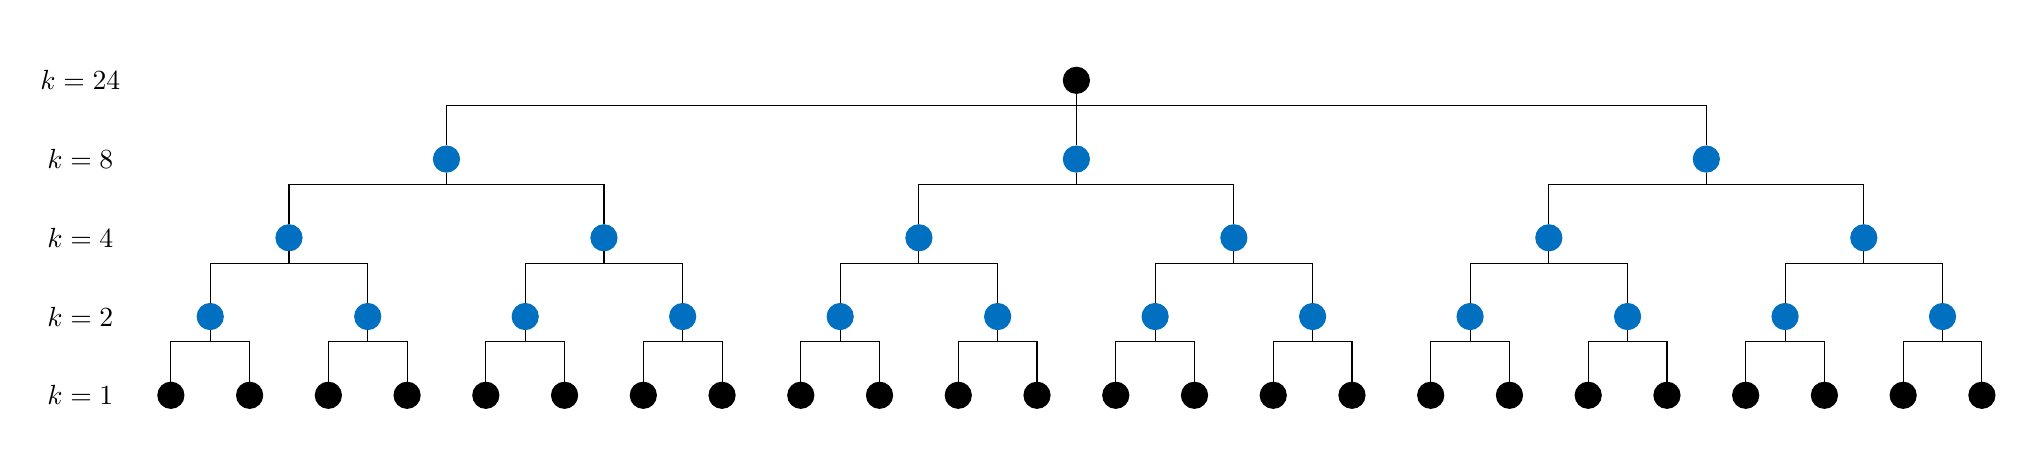
\begin{tikzpicture}[baseline=(current  bounding  box.center), every node/.append style={shape=circle, align = center, draw=newblue}]
	\node[draw = none] at (-0.15, 0) {$k = 1$};
	\node[draw = none] at (-0.15, 1) {$k = 2$};
	\node[draw = none] at (-0.15, 2) {$k = 4$};
	\node[draw = none] at (-0.15, 3) {$k = 8$};
	\node[draw = none] at (-0.15, 4) {$k = 24$};
		\foreach \x in {1,...,24}
			\node[fill = black, draw=black] at (\x, 0) (n\x){};
		\foreach \x in {2,4,...,24}
			\node[fill = newblue] at (\x-0.5, 1) (l\x){};
		\foreach \x in {3,7,...,24}
			\node[fill = newblue] at (\x-0.5, 2) (p\x){};
		\foreach \x in {5,13,...,24}
			\node[fill = newblue] at (\x-0.5, 3) (z\x){};
		\node[fill = black, draw=black] at (12.5, 4) (d24){};
		\foreach \x in {5,13,...,24}
			\relation{0.15}{z\x}{d24};
		\foreach \x in {3,7,...,24} {
			\pgfmathtruncatemacro{\j}{\x+1};
			\relation{0.15}{l\j}{p\x};
			\pgfmathtruncatemacro{\j}{\x-1};
			\relation{0.15}{l\j}{p\x};
		};
		\foreach \x in {5,13,...,24} {
			\pgfmathtruncatemacro{\j}{\x+2};
			\relation{0.15}{p\j}{z\x};
			\pgfmathtruncatemacro{\j}{\x-2};
			\relation{0.15}{p\j}{z\x};
		};
		\foreach \x in {2,4,...,24} {
			\pgfmathtruncatemacro{\j}{\x};
			\relation{0.15}{n\j}{l\x};
			\pgfmathtruncatemacro{\j}{\x-1};
			\relation{0.15}{n\j}{l\x};
		};
	\end{tikzpicture}}\\
{\scriptsize Temporal hierarchy $\{24, {\color{newred}12, 6, 3}, 1\}$}\\[-0.2cm]
\resizebox{\linewidth}{!}{
	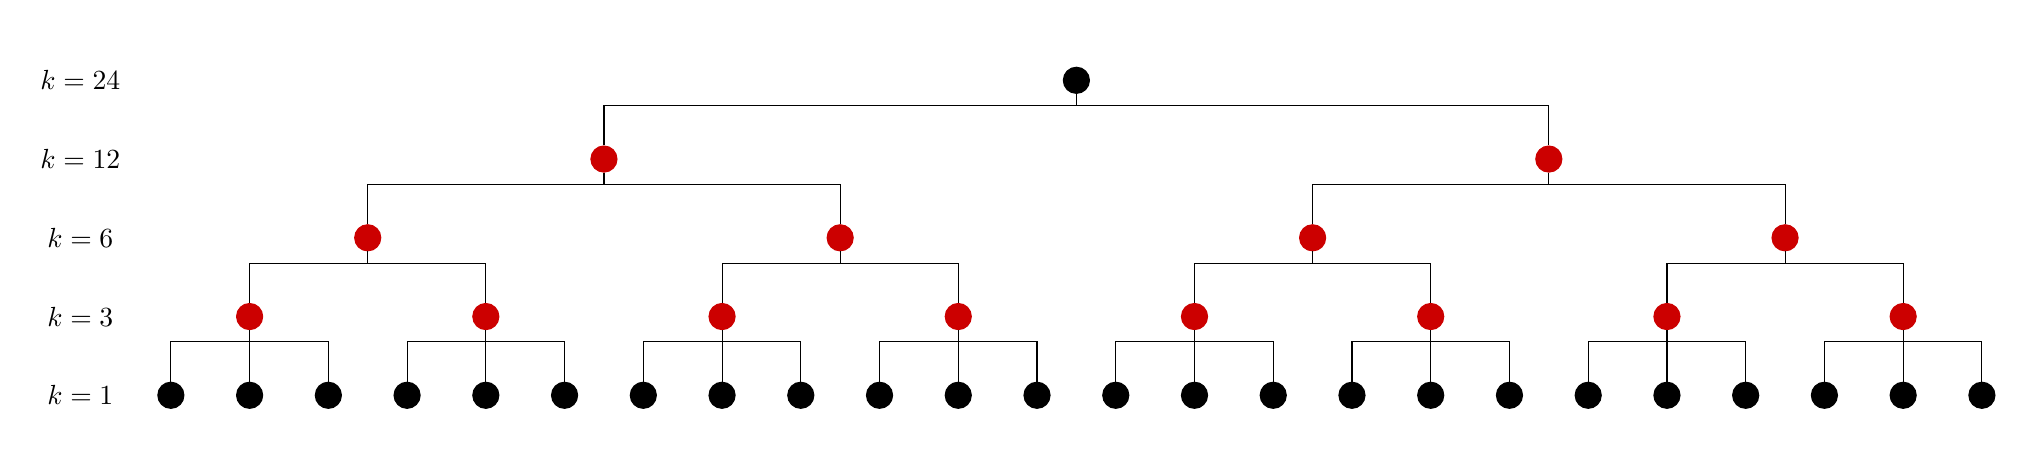
\begin{tikzpicture}[baseline=(current  bounding  box.center), every node/.append style={shape=circle, align = center, draw=newred}]
	\node[draw = none] at (-0.15, 0) {$k = 1$};
	\node[draw = none] at (-0.15, 1) {$k = 3$};
	\node[draw = none] at (-0.15, 2) {$k = 6$};
	\node[draw = none] at (-0.15, 3) {$k = 12$};
	\node[draw = none] at (-0.15, 4) {$k = 24$};
		\foreach \x in {1,...,24}
			\node[fill = black, draw=black] at (\x, 0) (n\x){};
		\foreach \x in {2,5,...,24}
			\node[fill = newred] at (\x, 1) (l\x){};
		\foreach \x in {4,10,...,24}
			\node[fill = newred] at (\x-0.5, 2) (p\x){};
		\foreach \x in {7, 19}
			\node[fill = newred] at (\x-0.5, 3) (z\x){};
		\node[fill = black, draw=black] at (12.5, 4) (d24){};
		\foreach \x in {7, 19}
			\relation{0.15}{z\x}{d24};
		\foreach \x in {7, 19} {
			\pgfmathtruncatemacro{\j}{\x-3};
			\relation{0.15}{p\j}{z\x};
			\pgfmathtruncatemacro{\j}{\x+3};
			\relation{0.15}{p\j}{z\x};
		};
		\foreach \x in {4,10,...,24} {
			\pgfmathtruncatemacro{\j}{\x-2};
			\relation{0.15}{l\j}{p\x};
			\pgfmathtruncatemacro{\j}{\x+1};
			\relation{0.15}{l\j}{p\x};
		};
		
		\foreach \x in {2,5,...,24} {
			\pgfmathtruncatemacro{\j}{\x-1};
			\relation{0.15}{n\j}{l\x};
			\pgfmathtruncatemacro{\j}{\x+1};
			\relation{0.15}{n\j}{l\x};
			\pgfmathtruncatemacro{\j}{\x};
			\relation{0.15}{n\j}{l\x};
		};
	\end{tikzpicture}}
\end{frame}
\end{document}
